%=================================================================
% CSE 4345 — Big Data Analytics
% Week 3, Part 1: The Big Data Ecosystem — HDFS, Hadoop,
%                 and the Distributed Storage Foundation
% Department of CSE, Premier University
%
% Part 1 covers: Architecture motivation · Hadoop ecosystem stack
%               · HDFS architecture (NameNode, DataNode, Secondary NN)
%               · Block storage & rack-aware replication
%               · Read/Write paths · HA · Ivy League alignment · Assessment
% Part 2 covers: GFS paper (Ghemawat et al., 2003) · Yahoo! case study
%=================================================================

\documentclass[aspectratio=169,10pt]{beamer}

%---------- Packages ----------
\usepackage[utf8]{inputenc}
\usepackage[T1]{fontenc}
\usepackage{booktabs}
\usepackage{xcolor}
\usepackage{tikz}
\usetikzlibrary{shapes.geometric, positioning, arrows.meta,
                decorations.pathreplacing, calc, fit, backgrounds}
\usepackage{amsmath}
\usepackage{graphicx}
\usepackage{multicol}
\usepackage{enumerate}
\usepackage{array}
\usepackage{listings}

%---------- Theme ----------
\usetheme{Madrid}

%---------- Premier University Color Identity ----------
\definecolor{PUNavy}{RGB}{10,36,99}
\definecolor{PUGold}{RGB}{197,151,37}
\definecolor{PULightBlue}{RGB}{210,228,255}
\definecolor{PUTeal}{RGB}{0,100,100}
\definecolor{PUGray}{RGB}{90,90,90}
\definecolor{PURed}{RGB}{160,30,30}
\definecolor{PUGreen}{RGB}{30,120,60}
\definecolor{PUOrange}{RGB}{200,100,20}
\definecolor{PUPurple}{RGB}{80,0,120}

\setbeamercolor{palette primary}{bg=PUNavy, fg=white}
\setbeamercolor{palette secondary}{bg=PUNavy!85, fg=white}
\setbeamercolor{palette tertiary}{bg=PUNavy!70, fg=white}
\setbeamercolor{palette quaternary}{bg=PUNavy, fg=white}
\setbeamercolor{structure}{fg=PUNavy}
\setbeamercolor{title}{bg=PUNavy, fg=PUGold}
\setbeamercolor{subtitle}{fg=white}
\setbeamercolor{frametitle}{bg=PUNavy, fg=PUGold}
\setbeamercolor{alerted text}{fg=PUGold!85!black}
\setbeamercolor{block title}{bg=PUNavy, fg=white}
\setbeamercolor{block body}{bg=PULightBlue!45}
\setbeamercolor{block title alerted}{bg=PUGold!80!black, fg=white}
\setbeamercolor{block body alerted}{bg=PUGold!12}
\setbeamercolor{block title example}{bg=PUTeal, fg=white}
\setbeamercolor{block body example}{bg=PUTeal!10}
\setbeamercolor{section in toc}{fg=PUNavy}
\setbeamercolor{itemize item}{fg=PUGold!80!black}
\setbeamercolor{itemize subitem}{fg=PUNavy!70}

\setbeamertemplate{navigation symbols}{}
\setbeamertemplate{itemize item}{\scriptsize\raise1.5pt\hbox{\textbullet}}
\setbeamertemplate{itemize subitem}{\scriptsize\raise1pt\hbox{--}}

%---------- Code listing style ----------
\lstset{
  basicstyle=\ttfamily\scriptsize,
  backgroundcolor=\color{PUNavy!8},
  frame=single,
  rulecolor=\color{PUNavy!30},
  breaklines=true,
  keywordstyle=\color{PUNavy}\bfseries,
  commentstyle=\color{PUGray}\itshape,
}

%---------- Section separator ----------
\AtBeginSection[]{
  \begin{frame}[plain]
    \vfill
    \centering
    \begin{beamercolorbox}[sep=12pt,center,shadow=true,rounded=true]{block title}
      \usebeamerfont{title}\insertsectionhead\par
    \end{beamercolorbox}
    \vfill
  \end{frame}
}

%---------- Title metadata ----------
\title[CSE 4345 \textbar{} Week 3, Part 1]{CSE 4345: Big Data Analytics}
\subtitle{Week 3, Part 1 \textemdash\ The Big Data Ecosystem: HDFS \&
          the Distributed Storage Foundation}
\author[Dept.\ of CSE]{Department of Computer Science \& Engineering\\[4pt]
       \small Premier University, Chittagong}
\institute{}
\date{Semester 2026}

%=================================================================
\begin{document}
%=================================================================

%----------------------------------------------------------------
% TITLE SLIDE
%----------------------------------------------------------------
\begin{frame}
  \titlepage
\end{frame}

%----------------------------------------------------------------
% COURSE INFO
%----------------------------------------------------------------
\begin{frame}{Course \& Lecture Information}
  \begin{columns}[T]
    \column{0.47\textwidth}
      \begin{block}{Lecture Identity}
        \begin{tabular}{ll}
          \textbf{Course:}      & CSE 4345 \\
          \textbf{Week / Part:} & 3 of 11 \textbar\ Part 1 of 2 \\
          \textbf{CLO:}         & CLO1 \\
          \textbf{PLO:}         & PLO(a) \\
        \end{tabular}
      \end{block}
      \vspace{6pt}
      \begin{alertblock}{CLO1}
        \textit{``Understand big data characteristics''}
      \end{alertblock}
      \vspace{6pt}
      \begin{block}{Course Progression}
        \small
        Week 1: \textit{What} is Big Data (3Vs)\\
        Week 2: \textit{Why} integration is hard\\
        \textbf{Week 3: \textit{Where} data is stored (HDFS)}\\
        Week 4: \textit{How} data is processed (MapReduce)
      \end{block}

    \column{0.50\textwidth}
      \begin{exampleblock}{Part 1 Covers}
        \begin{itemize}
          \item The architecture shift: RDBMS $\to$ distributed storage
          \item The core principle: move computation to data
          \item The Hadoop ecosystem stack (layered)
          \item HDFS: NameNode, DataNode, Secondary NameNode
          \item Block storage and rack-aware replication
          \item HDFS read \& write paths
          \item High availability (Active / Standby NameNode)
          \item The small file problem
          \item Ivy League alignment
          \item Student assessment pool
        \end{itemize}
      \end{exampleblock}
  \end{columns}
\end{frame}

%----------------------------------------------------------------
% AGENDA
%----------------------------------------------------------------
\begin{frame}{Lecture Agenda}
  \tableofcontents
\end{frame}

%================================================================
\section{The Architecture Motivation}
%================================================================

\begin{frame}{Why a New Storage Architecture?}
  \begin{columns}[T]
    \column{0.52\textwidth}
      \begin{block}{The 2003 Problem Statement}
        Google's web crawl produced petabytes of data that needed to be:
        \begin{itemize}
          \item \textbf{Stored} reliably across thousands of machines
          \item \textbf{Queried} for web indexing (sequential scans of entire datasets)
          \item \textbf{Fault-tolerant}: hardware failure expected daily at this scale
          \item \textbf{Cheap}: commodity PCs, not mainframes
        \end{itemize}
      \end{block}
      \vspace{6pt}
      \begin{alertblock}{What Existing Systems Could NOT Do}
        \begin{itemize}
          \item \textbf{NFS / POSIX FS}: single server, no horizontal scale
          \item \textbf{RDBMS}: tuned for random access, not sequential petabyte scans
          \item \textbf{SAN / NAS}: expensive proprietary hardware; single point of failure
        \end{itemize}
      \end{alertblock}

    \column{0.45\textwidth}
      \begin{exampleblock}{The Paradigm Shift}
        \begin{center}
        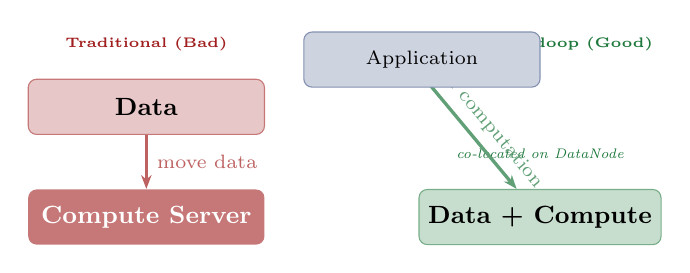
\begin{tikzpicture}[
            box/.style={rectangle, rounded corners=3pt,
                        minimum width=3.0cm, minimum height=0.7cm,
                        align=center, font=\small\bfseries},
            arr/.style={-{Stealth[length=5pt]}, very thick}
          ]
          % Old way
          \node[box, fill=PURed!25, draw=PURed!60] (data)  at (0,  2.2)
                {Data};
          \node[box, fill=PURed!60, text=white]     (comp)  at (0,  0.8)
                {Compute Server};
          \draw[arr, PURed!70] (data) -- node[right, font=\scriptsize]{move data} (comp);
          \node[font=\tiny\bfseries, PURed] at (0, 3.0) {Traditional (Bad)};

          % New way
          \node[box, fill=PUGreen!25, draw=PUGreen!60] (data2) at (5,  0.8)
                {Data + Compute};
          \node[font=\tiny\itshape, PUGreen] at (5, 1.6)
                {co-located on DataNode};
          \draw[arr, PUGreen!70] (3.5, 2.6)
                -- node[above, font=\scriptsize, sloped]{send computation} (data2);
          \node[font=\tiny\bfseries, PUGreen] at (5, 3.0) {HDFS / Hadoop (Good)};

          \node[box, fill=PUNavy!20, draw=PUNavy!50, font=\scriptsize]
                (app) at (3.5, 2.8) {Application};
        \end{tikzpicture}
        \end{center}
      \end{exampleblock}
      \vspace{4pt}
      \begin{block}{The Fundamental Insight}
        \small \textbf{Moving computation is cheaper than moving data.}  A 100 GB input file costs seconds to process locally; copying it over a network costs minutes.
      \end{block}
  \end{columns}
\end{frame}

%----------------------------------------------------------------
\begin{frame}{The Core Principle: Data Locality}
  \begin{columns}[T]
    \column{0.55\textwidth}
      \begin{block}{Definition: Data Locality}
        Running computation \textbf{on the same physical node} that holds the required data, avoiding network transfer.
      \end{block}
      \vspace{6pt}
      \textbf{Network transfer cost (2024 estimates):}
      \vspace{4pt}
      \renewcommand{\arraystretch}{1.25}
      \begin{tabular}{p{3.0cm}r}
        \toprule
        \textbf{Transfer medium} & \textbf{Throughput} \\
        \midrule
        Local disk read (SSD)    & $\sim$3{,}000 MB/s \\
        Local disk read (HDD)    & $\sim$150 MB/s \\
        Intra-rack network (1G)  & $\sim$125 MB/s \\
        Cross-rack network (1G)  & $\sim$100 MB/s \\
        Cross-datacenter WAN     & $\sim$10 MB/s \\
        \bottomrule
      \end{tabular}
      \vspace{6pt}
      \begin{alertblock}{Consequence}
        For a 500 GB file, local disk is \textbf{3--300$\times$ faster} than any network path.  HDFS + MapReduce/Spark schedule tasks on the node that \emph{owns} the data, achieving near-local speed at petabyte scale.
      \end{alertblock}

    \column{0.42\textwidth}
      \begin{exampleblock}{Three Levels of Locality (MapReduce / YARN)}
        \vspace{4pt}
        \begin{enumerate}
          \item \textbf{Data-local}: Task runs on the \emph{same node} as the block
          \begin{itemize}
            \scriptsize\item Best case: no network I/O
          \end{itemize}
          \vspace{4pt}
          \item \textbf{Rack-local}: Task runs on a \emph{different node in the same rack}
          \begin{itemize}
            \scriptsize\item One hop through top-of-rack switch
          \end{itemize}
          \vspace{4pt}
          \item \textbf{Off-rack}: Task runs on a \emph{different rack}
          \begin{itemize}
            \scriptsize\item Crosses the core network; worst case
          \end{itemize}
        \end{enumerate}
        \vspace{4pt}
        YARN's scheduler tries level 1 first, falls back to level 2, then 3.
      \end{exampleblock}
      \vspace{4pt}
      \begin{block}{GFS Paper (2003)}
        \textit{``We have optimised for large sequential reads and the cases where computation and data co-reside on the same machine.''}
      \end{block}
  \end{columns}
\end{frame}

%================================================================
\section{The Hadoop Ecosystem Stack}
%================================================================

\begin{frame}{The Hadoop Ecosystem: Layered Architecture}
  \begin{center}
  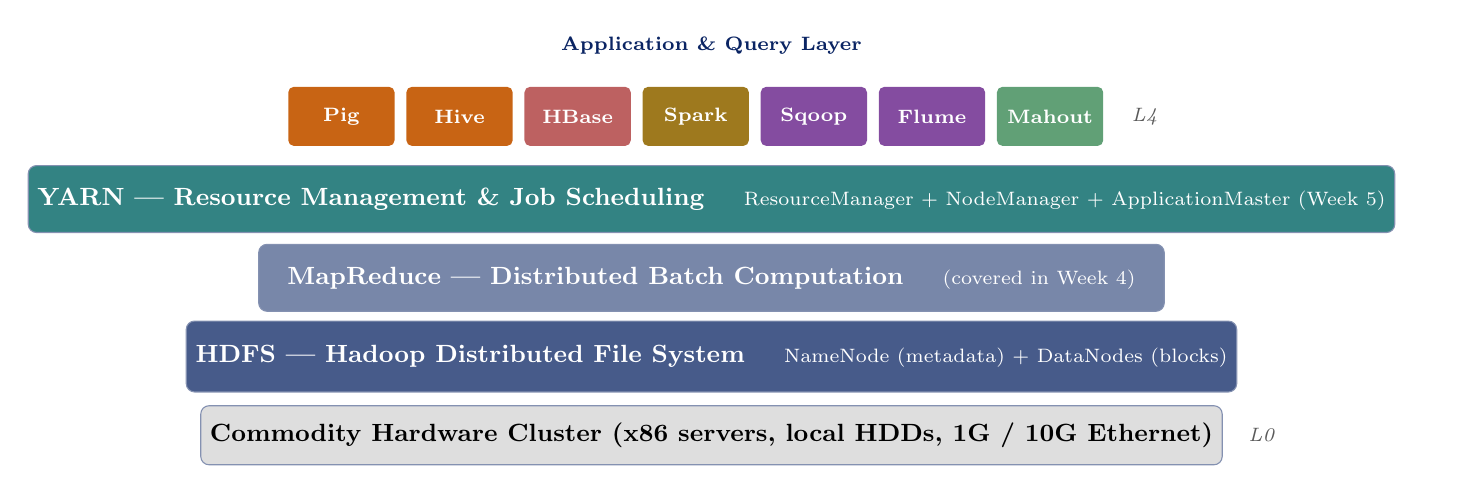
\begin{tikzpicture}[
      layer/.style={rectangle, draw=PUNavy!50, rounded corners=3pt,
                    minimum width=11.5cm, align=center, font=\small\bfseries},
      lbl/.style={font=\scriptsize\itshape, PUGray}
    ]
    % Layer 0 — Hardware
    \node[layer, minimum height=0.75cm, fill=PUGray!20]
          (hw) at (0, 0)
          {Commodity Hardware Cluster (x86 servers, local HDDs, 1G / 10G Ethernet)};
    \node[lbl, right=0.2cm of hw] {L0};

    % Layer 1 — HDFS
    \node[layer, minimum height=0.9cm, fill=PUNavy!75, text=white]
          (hdfs) at (0, 1.0)
          {HDFS — Hadoop Distributed File System \quad
           {\normalfont\scriptsize NameNode (metadata) + DataNodes (blocks)}};
    \node[lbl, right=0.2cm of hdfs, text=white] {L1};

    % Layer 2 — Compute
    \node[layer, minimum height=0.85cm, fill=PUNavy!55, text=white]
          (mr) at (0, 2.0)
          {MapReduce — Distributed Batch Computation \quad
           {\normalfont\scriptsize (covered in Week 4)}};
    \node[lbl, right=0.2cm of mr, text=white] {L2};

    % Layer 3 — YARN
    \node[layer, minimum height=0.85cm, fill=PUTeal!80, text=white]
          (yarn) at (0, 3.0)
          {YARN — Resource Management \& Job Scheduling \quad
           {\normalfont\scriptsize ResourceManager + NodeManager + ApplicationMaster (Week 5)}};
    \node[lbl, right=0.2cm of yarn, text=white] {L3};

    % Layer 4 — Apps (multiple boxes)
    \begin{scope}[shift={(0, 4.05)}]
      \foreach \x/\name/\col in {
        -4.7/Pig/PUOrange,
        -3.2/Hive/PUOrange,
        -1.7/HBase/PURed!70,
        -0.2/Spark/PUGold!80!black,
         1.3/Sqoop/PUPurple!70,
         2.8/Flume/PUPurple!70,
         4.3/Mahout/PUGreen!70
      }{
        \node[rectangle, rounded corners=2pt,
              fill=\col, text=white,
              minimum width=1.35cm, minimum height=0.75cm,
              font=\scriptsize\bfseries]
              at (\x, 0) {\name};
      }
    \end{scope}
    \node[lbl] at (5.5, 4.05) {L4};

    % Brace or label for L4
    \node[font=\scriptsize\bfseries, PUNavy] at (0, 4.95)
          {Application \& Query Layer};
  \end{tikzpicture}
  \end{center}
  \vspace{2pt}
  \begin{alertblock}{Design Philosophy}
    Each layer is \textbf{independently replaceable}.  YARN replaced MapReduce's resource manager in Hadoop 2.0, allowing Spark, Tez, and Storm to share the same HDFS cluster without rewriting data storage.
  \end{alertblock}
\end{frame}

%----------------------------------------------------------------
\begin{frame}{Ecosystem Components: Roles at a Glance}
  \centering
  \renewcommand{\arraystretch}{1.38}
  \begin{tabular}{p{1.8cm}p{1.5cm}p{7.0cm}}
    \toprule
    \textbf{Component} & \textbf{Week} & \textbf{Role} \\
    \midrule
    \textbf{HDFS}      & 3 & Distributed file system; stores data as blocks across DataNodes \\
    \textbf{MapReduce} & 4 & Parallel batch computation model (Map + Shuffle + Reduce) \\
    \textbf{YARN}      & 5 & Cluster resource manager; schedules CPU/RAM across all frameworks \\
    \textbf{Pig}       & 4 & Dataflow scripting language (Pig Latin) for ETL pipelines \\
    \textbf{Hive}      & 7 & SQL-on-Hadoop; translates HiveQL to MapReduce / Spark jobs \\
    \textbf{HBase}     & 4 & NoSQL column-family store for low-latency random read/write \\
    \textbf{Spark}     & 6 & In-memory distributed computing; 10--100$\times$ faster than MapReduce \\
    \textbf{Sqoop}     & 8 & Bulk transfer between RDBMS (MySQL/Oracle) and HDFS \\
    \textbf{Flume}     & 8 & Streaming log/event ingest into HDFS \\
    \textbf{Mahout}    & -- & Distributed machine learning algorithms on Hadoop \\
    \bottomrule
  \end{tabular}
  \vspace{6pt}
  \begin{block}{Key Takeaway}
    HDFS is the \textbf{foundation} every other component builds on.  Understanding HDFS deeply is a prerequisite for all subsequent weeks.
  \end{block}
\end{frame}

%----------------------------------------------------------------
\begin{frame}{The Economics of Commodity Hardware}
  \begin{columns}[T]
    \column{0.52\textwidth}
      \begin{block}{Google's Original Design Mandate (GFS, 2003)}
        \textit{``The system is built from many inexpensive commodity components that often fail.  It must constantly monitor itself, detect, tolerate, and recover promptly from component failures.''}
      \end{block}
      \vspace{6pt}
      \textbf{Failure rates at scale:}
      \vspace{4pt}
      \renewcommand{\arraystretch}{1.2}
      \begin{tabular}{lr}
        \toprule
        \textbf{Failure type} & \textbf{Rate (per year)} \\
        \midrule
        Individual disk failure    & 2--4\% \\
        Individual server failure  & 5--10\% \\
        Power supply failure       & 1--2\% \\
        Rack switch failure        & 0.5--1\% \\
        \midrule
        \textbf{In a 1{,}000-node cluster} & \textbf{50--100 failures/year} \\
        \bottomrule
      \end{tabular}

    \column{0.45\textwidth}
      \begin{alertblock}{Design Consequence}
        At 1{,}000+ nodes, hardware failure is not an \textbf{exception}\textemdash it is \textbf{routine}.  HDFS must handle failures \emph{transparently} without operator intervention or data loss.
      \end{alertblock}
      \vspace{6pt}
      \begin{exampleblock}{Cost Comparison (2024 estimates)}
        \small
        \begin{tabular}{lrr}
          \toprule
          & \textbf{SAN Array} & \textbf{HDFS Cluster} \\
          \midrule
          Storage (1 PB)  & \$500K+ & \$50K \\
          Redundancy      & RAID     & 3$\times$ replication \\
          Scalability     & Vendor   & Add nodes\\
          Lock-in         & High     & None \\
          \bottomrule
        \end{tabular}
        \vspace{4pt}
        HDFS achieves \textbf{10$\times$ cost reduction} while adding fault tolerance by design.
      \end{exampleblock}
  \end{columns}
\end{frame}

%================================================================
\section{HDFS: Architecture \& Design}
%================================================================

\begin{frame}{HDFS Master / Worker Architecture}
  \begin{columns}[T]
    \column{0.48\textwidth}
      \begin{block}{Three Core Components}
        \begin{itemize}
          \item \textbf{NameNode} (1 active): the master.  Stores all filesystem \emph{metadata} in RAM.
          \item \textbf{DataNode} ($n$ workers): the storage nodes.  Store actual data \emph{blocks} on local disks.
          \item \textbf{Secondary NameNode} (1): performs periodic metadata checkpointing.  \alert{NOT} a failover.
        \end{itemize}
      \end{block}
      \vspace{4pt}
      \begin{alertblock}{Two Distinct Planes}
        \begin{itemize}
          \item \textbf{Metadata plane}: Client $\leftrightarrow$ NameNode\\(file names, block locations, permissions)
          \item \textbf{Data plane}: Client $\leftrightarrow$ DataNode\\(actual bytes read / written)
        \end{itemize}
        Separating these planes is a \textbf{critical design choice}: NameNode never touches data, so it can serve thousands of clients simultaneously.
      \end{alertblock}

    \column{0.49\textwidth}
      \begin{center}
      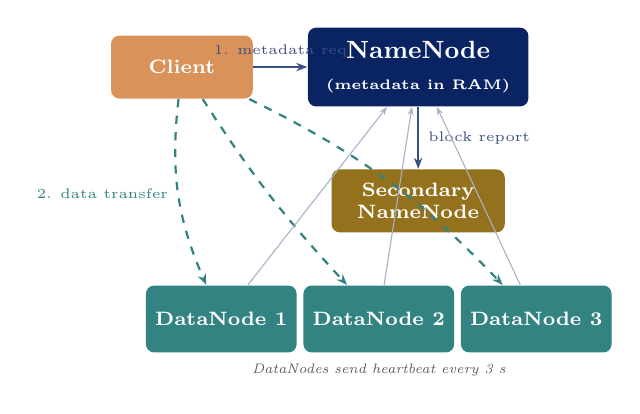
\begin{tikzpicture}[
          nn/.style={rectangle, rounded corners=3pt, fill=PUNavy,
                     text=white, minimum width=2.8cm, minimum height=1.0cm,
                     font=\small\bfseries, align=center},
          dn/.style={rectangle, rounded corners=3pt, fill=PUTeal!80,
                     text=white, minimum width=1.6cm, minimum height=0.85cm,
                     font=\scriptsize\bfseries, align=center},
          snn/.style={rectangle, rounded corners=3pt, fill=PUGold!75!black,
                      text=white, minimum width=2.2cm, minimum height=0.8cm,
                      font=\scriptsize\bfseries, align=center},
          cl/.style={rectangle, rounded corners=3pt, fill=PUOrange!70,
                     text=white, minimum width=1.8cm, minimum height=0.8cm,
                     font=\scriptsize\bfseries, align=center},
          meta/.style={-{Stealth[length=4pt]}, PUNavy!80, thick},
          data/.style={-{Stealth[length=4pt]}, PUTeal!80, thick, dashed}
        ]
        % Client
        \node[cl]  (cli)  at (0,   3.5) {Client};
        % NameNode
        \node[nn]  (nn)   at (3.0, 3.5) {NameNode\\{\tiny (metadata in RAM)}};
        % Secondary NN
        \node[snn] (snn)  at (3.0, 1.8) {Secondary\\NameNode};
        % DataNodes
        \node[dn]  (dn1)  at (0.5, 0.3) {DataNode 1};
        \node[dn]  (dn2)  at (2.5, 0.3) {DataNode 2};
        \node[dn]  (dn3)  at (4.5, 0.3) {DataNode 3};

        % Metadata arrows
        \draw[meta] (cli) -- node[above, font=\tiny]{1. metadata req} (nn);
        \draw[meta] (nn)  -- node[right, font=\tiny]{block report} (snn);

        % Data arrows
        \draw[data] (cli) to[bend right=15]
              node[left, font=\tiny]{2. data transfer} (dn1);
        \draw[data] (cli) to[bend right=5] (dn2);
        \draw[data] (cli) to[bend left=10] (dn3);

        % Heartbeat arrows from DNs to NN
        \draw[-{Stealth[length=3pt]}, PUNavy!35, thin]
              (dn1) -- (nn);
        \draw[-{Stealth[length=3pt]}, PUNavy!35, thin]
              (dn2) -- (nn);
        \draw[-{Stealth[length=3pt]}, PUNavy!35, thin]
              (dn3) -- (nn);
        \node[font=\tiny\itshape, PUGray] at (2.5,-0.35)
              {DataNodes send heartbeat every 3 s};
      \end{tikzpicture}
      \end{center}
  \end{columns}
\end{frame}

%----------------------------------------------------------------
\begin{frame}{NameNode: The Brain of HDFS}
  \begin{columns}[T]
    \column{0.52\textwidth}
      \begin{block}{What the NameNode Stores (in RAM)}
        \begin{itemize}
          \item \textbf{Namespace tree}: complete directory hierarchy of all files and directories
          \item \textbf{File $\to$ block mapping}: for each file, which blocks it consists of, in order
          \item \textbf{Block $\to$ DataNode mapping}: where each block replica is currently stored (rebuilt from DataNode reports at startup)
          \item \textbf{Permissions}: POSIX-style owner, group, access rights
        \end{itemize}
      \end{block}
      \vspace{4pt}
      \begin{alertblock}{Why RAM? Why Dangerous?}
        In-memory metadata = \textbf{microsecond lookups} (vs.\ disk-based = milliseconds).  But: the NameNode is a \textbf{single point of failure}.  If it crashes, the entire cluster is inaccessible until recovered.
      \end{alertblock}

    \column{0.45\textwidth}
      \begin{exampleblock}{NameNode Metadata Persistence}
        \begin{center}
        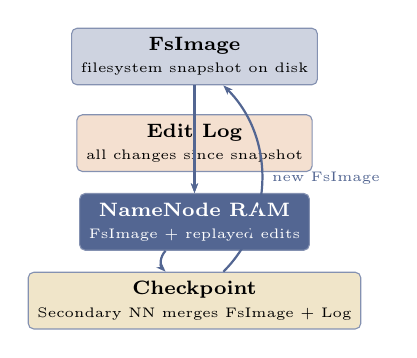
\begin{tikzpicture}[
            box/.style={rectangle, rounded corners=2pt, draw=PUNavy!50,
                        minimum width=2.6cm, minimum height=0.7cm,
                        font=\scriptsize, align=center},
            arr/.style={-{Stealth[length=3.5pt]}, PUNavy!70, thick}
          ]
          \node[box, fill=PUNavy!20] (fs)  at (0, 2.8) {\textbf{FsImage}\\{\tiny filesystem snapshot on disk}};
          \node[box, fill=PUOrange!20] (el) at (0, 1.7) {\textbf{Edit Log}\\{\tiny all changes since snapshot}};
          \node[box, fill=PUNavy!70, text=white] (nn) at (0, 0.7)
                {\textbf{NameNode RAM}\\{\tiny FsImage $+$ replayed edits}};
          \node[box, fill=PUGold!25] (cp) at (0, -0.3)
                {\textbf{Checkpoint}\\{\tiny Secondary NN merges FsImage $+$ Log}};

          \draw[arr] (fs)  -- (nn);
          \draw[arr] (el)  -- (nn);
          \draw[arr] (nn)  to[bend right=45] (cp);
          \draw[arr] (cp)  to[bend right=45]
                node[right, font=\tiny]{new FsImage} (fs);
        \end{tikzpicture}
        \end{center}
      \end{exampleblock}
      \vspace{4pt}
      \begin{block}{Startup Sequence}
        \small NameNode loads \textbf{FsImage} from disk $\to$ replays all \textbf{Edit Log} entries $\to$ waits for DataNodes to report block locations $\to$ enters \emph{safe mode} until replication factor is met.
      \end{block}
  \end{columns}
\end{frame}

%----------------------------------------------------------------
\begin{frame}{Secondary NameNode: The Critical Misconception}
  \begin{columns}[T]
    \column{0.52\textwidth}
      \begin{alertblock}{Common Exam Mistake}
        \textbf{The Secondary NameNode is NOT a failover!}\\[4pt]
        Its name is misleading.  If the active NameNode crashes, the Secondary NameNode \textbf{cannot automatically take over}.  The cluster goes down.
      \end{alertblock}
      \vspace{6pt}
      \begin{block}{What It Actually Does: Checkpointing}
        \begin{enumerate}
          \item Periodically fetches the current \textbf{FsImage} and \textbf{Edit Log} from NameNode
          \item Merges them into a new, compact \textbf{FsImage}
          \item Pushes the merged FsImage back to NameNode
          \item Clears the Edit Log on NameNode
        \end{enumerate}
        \vspace{4pt}
        \textbf{Why needed?}  Without checkpointing, the Edit Log grows indefinitely, making NameNode restart slower and slower (it must replay the entire log).
      \end{block}

    \column{0.45\textwidth}
      \begin{exampleblock}{Analogy: Bank Ledger}
        \small
        \begin{itemize}
          \item \textbf{FsImage} = the bank's \emph{balance sheet} (snapshot at end of month)
          \item \textbf{Edit Log} = the bank's \emph{transaction journal} (every deposit/withdrawal this month)
          \item \textbf{Secondary NameNode} = the \emph{accountant} who reconciles the journal into a new balance sheet at month-end, reducing the journal to zero
          \item Without the accountant, the journal grows without bound and takes longer to audit each time
        \end{itemize}
      \end{exampleblock}
      \vspace{4pt}
      \begin{block}{True Failover: HDFS HA (Hadoop 2.0+)}
        \small \textbf{Active NameNode} + \textbf{Standby NameNode} share a \textbf{Quorum Journal Manager} (3+ JournalNodes).  Standby replays edits in real time.  On failover: ZooKeeper triggers automatic switch in $<$30 seconds.
      \end{block}
  \end{columns}
\end{frame}

%----------------------------------------------------------------
\begin{frame}{DataNode: Block Storage in Practice}
  \begin{columns}[T]
    \column{0.52\textwidth}
      \begin{block}{What a DataNode Does}
        \begin{itemize}
          \item Stores data as \textbf{flat files on local disk} (one file per HDFS block)
          \item Sends a \textbf{heartbeat} to NameNode every 3 seconds (liveness signal)
          \item Sends a \textbf{block report} to NameNode every 6 hours (full inventory of stored blocks)
          \item Serves \textbf{client read requests} directly (no NameNode involved in data transfer)
          \item Participates in \textbf{replication pipeline} for writes
          \item Runs \textbf{block scanner} to detect silent bit-rot (checksum verification)
        \end{itemize}
      \end{block}
      \vspace{4pt}
      \begin{alertblock}{NameNode Detection of DataNode Failure}
        If a DataNode misses \textbf{10 consecutive heartbeats} (30 seconds), NameNode marks it as dead and schedules re-replication of all under-replicated blocks.
      \end{alertblock}

    \column{0.45\textwidth}
      \begin{exampleblock}{Block Storage: How a 300 MB File is Stored}
        \begin{center}
        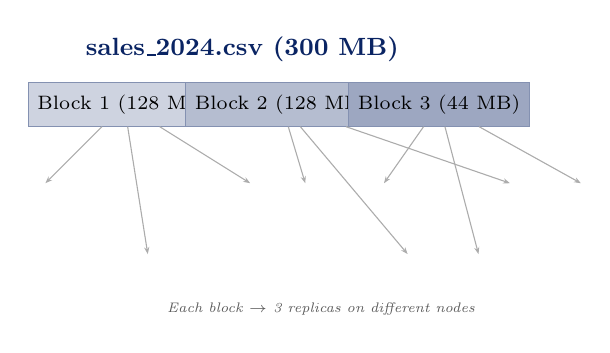
\begin{tikzpicture}[
            blk/.style={rectangle, draw=PUNavy!50, minimum width=2.2cm,
                        minimum height=0.55cm, font=\scriptsize, align=center},
            dn/.style={rectangle, rounded corners=2pt,
                       fill=PUTeal!20, draw=PUTeal!60,
                       minimum width=2.4cm, minimum height=0.6cm,
                       font=\scriptsize\bfseries}
          ]
          \node[font=\small\bfseries, PUNavy] at (0,3.2) {sales\_2024.csv (300 MB)};
          \node[blk, fill=PUNavy!20]  (b1) at (-1.5,2.5) {Block 1 (128 MB)};
          \node[blk, fill=PUNavy!30]  (b2) at ( 0.5,2.5) {Block 2 (128 MB)};
          \node[blk, fill=PUNavy!40]  (b3) at ( 2.5,2.5) {Block 3 (44 MB)};

          % Replicas
          \foreach \b/\x/\y/\col in {
            b1/-2.5/1.4/PUTeal!60,
            b1/-1.2/0.5/PUTeal!60,
            b1/ 0.1/1.4/PUTeal!60,
            b2/ 0.8/1.4/PUNavy!40,
            b2/ 2.1/0.5/PUNavy!40,
            b2/ 3.4/1.4/PUNavy!40,
            b3/ 3.0/0.5/PURed!40,
            b3/ 4.3/1.4/PURed!40,
            b3/ 1.8/1.4/PURed!40
          }{
            \draw[-{Stealth[length=2.5pt]}, thin, PUGray!50] (\b) -- (\x,\y+0.1);
          }
          \node[font=\tiny\itshape, PUGray] at (1.0,-0.1)
                {Each block $\to$ 3 replicas on different nodes};
        \end{tikzpicture}
        \end{center}
      \end{exampleblock}
  \end{columns}
\end{frame}

%----------------------------------------------------------------
\begin{frame}{Block Size: Why 128 MB?}
  \begin{columns}[T]
    \column{0.52\textwidth}
      \begin{block}{Traditional Filesystem Block Size: 4 KB}
        In a traditional OS (ext4, NTFS):
        \begin{itemize}
          \item 4 KB block = minimise \emph{internal fragmentation} (wasted space within a block)
          \item Files are small (KB to MB range)
          \item \textbf{Random access} is common: seek to any byte quickly
        \end{itemize}
      \end{block}
      \vspace{6pt}
      \begin{exampleblock}{HDFS Block Size: 128 MB (default, Hadoop 2.x+)}
        In HDFS:
        \begin{itemize}
          \item Files are \textbf{large} (GB to TB): a 10 GB file = 80 blocks at 128 MB
          \item Workloads are \textbf{sequential reads}: MapReduce scans entire files
          \item Seek time is \textbf{negligible} relative to transfer time at 128 MB
          \item Fewer blocks = \textbf{fewer metadata entries} in NameNode RAM
        \end{itemize}
      \end{exampleblock}

    \column{0.45\textwidth}
      \begin{alertblock}{The Small File Problem}
        HDFS's Achilles' heel: if you store \textbf{millions of small files} (e.g., 1 KB each):
        \vspace{4pt}
        \begin{itemize}
          \item Each file $=$ at least 1 block $=$ 1 metadata entry in NameNode
          \item 10 million files $\approx$ \textbf{10 million metadata objects} in RAM
          \item NameNode RAM exhaustion $\to$ cluster unusable
          \item Each task processes only 1 KB but incurs full task-startup overhead
        \end{itemize}
        \vspace{4pt}
        \textbf{Solutions:}
        \begin{itemize}
          \small
          \item \textbf{HAR files}: bundle small files into a Hadoop Archive
          \item \textbf{SequenceFile}: merge small files into one large record file
          \item Ingest via \textbf{Kafka $\to$ micro-batch}: accumulate before writing to HDFS
        \end{itemize}
      \end{alertblock}
  \end{columns}
\end{frame}

%================================================================
\section{HDFS: Replication, Read \& Write Paths}
%================================================================

\begin{frame}{Rack-Aware Replication Strategy}
  \begin{columns}[T]
    \column{0.50\textwidth}
      \begin{block}{Default Replication Factor: 3}
        HDFS places three replicas of each block using a \textbf{rack-aware} policy to tolerate \emph{both} node failure and rack failure:
        \vspace{4pt}
        \begin{enumerate}
          \item \textbf{Replica 1}: Same node as the writer client (data-local write)
          \item \textbf{Replica 2}: A different node in a \emph{different rack} (off-rack)
          \item \textbf{Replica 3}: Another node in the \emph{same rack as Replica 2} (for intra-rack bandwidth)
        \end{enumerate}
      \end{block}
      \vspace{4pt}
      \begin{alertblock}{What Failures Are Tolerated?}
        \begin{itemize}
          \item \textbf{Any 1 node fails}: 2 replicas remain; replication restored automatically
          \item \textbf{Entire Rack 1 fails}: Replicas 2 and 3 survive on Rack 2
          \item \textbf{Any 2 nodes fail simultaneously}: 1 replica remains; urgent re-replication triggered
        \end{itemize}
      \end{alertblock}

    \column{0.47\textwidth}
      \begin{center}
      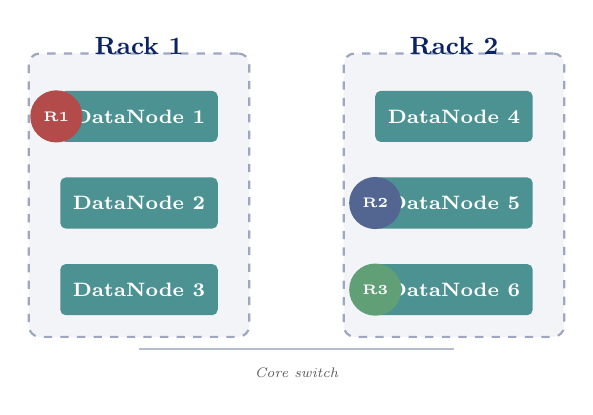
\begin{tikzpicture}[
          rack/.style={rectangle, rounded corners=4pt, draw=PUNavy!40,
                       dashed, thick, fill=PUNavy!5,
                       minimum width=2.8cm, minimum height=3.6cm},
          dn/.style={rectangle, rounded corners=2pt, fill=PUTeal!70,
                     text=white, minimum width=2.0cm, minimum height=0.65cm,
                     font=\scriptsize\bfseries},
          rep/.style={circle, fill=PUGold!80!black, text=white,
                      minimum size=0.45cm, font=\tiny\bfseries}
        ]
        % Rack 1
        \node[rack] (r1) at (0, 1.8) {};
        \node[font=\small\bfseries, PUNavy] at (0, 3.7) {Rack 1};
        \node[dn] (dn1) at (0, 2.8) {DataNode 1};
        \node[dn] (dn2) at (0, 1.7) {DataNode 2};
        \node[dn] (dn3) at (0, 0.6) {DataNode 3};

        % Rack 2
        \node[rack] (r2) at (4, 1.8) {};
        \node[font=\small\bfseries, PUNavy] at (4, 3.7) {Rack 2};
        \node[dn] (dn4) at (4, 2.8) {DataNode 4};
        \node[dn] (dn5) at (4, 1.7) {DataNode 5};
        \node[dn] (dn6) at (4, 0.6) {DataNode 6};

        % Replica badges
        \node[rep, fill=PURed!80]    at (-1.05, 2.8) {R1};
        \node[rep, fill=PUNavy!70]   at ( 3.0,  1.7) {R2};
        \node[rep, fill=PUGreen!70]  at ( 3.0,  0.6) {R3};

        % Switch
        \draw[PUNavy!30, thick] (0, -0.15) -- (4, -0.15);
        \node[font=\tiny\itshape, PUGray] at (2, -0.45) {Core switch};
      \end{tikzpicture}
      \end{center}
      \vspace{2pt}
      \begin{block}{\small Configuring Replication}
        \small Default: \texttt{dfs.replication=3}.  Change per-file: \texttt{hdfs dfs -setrep 2 /path/file}
      \end{block}
  \end{columns}
\end{frame}

%----------------------------------------------------------------
\begin{frame}[fragile]{HDFS Read Path}
  \begin{columns}[T]
    \column{0.50\textwidth}
      \begin{block}{Read Sequence (6 Steps)}
        \begin{enumerate}
          \item Client opens file via \textbf{DistributedFileSystem API}
          \item \textbf{NameNode} returns ordered list of block locations (sorted by network proximity to client)
          \item Client connects to the \textbf{closest DataNode} for Block 1 and reads it
          \item Client reads Block 1; \textbf{checksum} verified on each chunk
          \item Client moves to the next block $\to$ next-closest DataNode
          \item Process repeats until all blocks read; client closes the stream
        \end{enumerate}
      \end{block}
      \vspace{4pt}
      \begin{exampleblock}{Fault Handling During Read}
        If a DataNode fails mid-read, the client switches to the \textbf{next replica} for that block automatically.  The failed DataNode is blacklisted for the remainder of the read session.
      \end{exampleblock}

    \column{0.47\textwidth}
      \begin{center}
      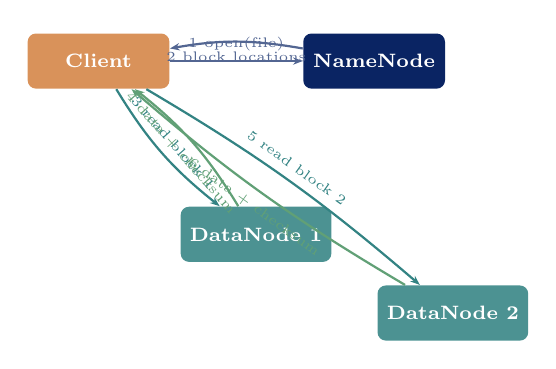
\begin{tikzpicture}[
          actor/.style={rectangle, rounded corners=3pt,
                        minimum width=1.8cm, minimum height=0.7cm,
                        font=\scriptsize\bfseries, align=center},
          arr/.style={-{Stealth[length=3.5pt]}, thick},
          lbl/.style={font=\tiny, sloped, above}
        ]
        \node[actor, fill=PUOrange!70, text=white] (cl) at (0,   5.0) {Client};
        \node[actor, fill=PUNavy,       text=white] (nn) at (3.5, 5.0) {NameNode};
        \node[actor, fill=PUTeal!70,    text=white] (d1) at (2.0, 2.8) {DataNode 1};
        \node[actor, fill=PUTeal!70,    text=white] (d2) at (4.5, 1.8) {DataNode 2};

        % Step lines
        \draw[arr, PUNavy!70]    (cl) -- node[lbl]{1~open(file)} (nn);
        \draw[arr, PUNavy!70]    (nn) to[bend right=10]
              node[lbl, below]{2~block locations} (cl);
        \draw[arr, PUTeal!80]    (cl) to[bend right=10]
              node[lbl]{3~read block 1} (d1);
        \draw[arr, PUGreen!70]   (d1) to[bend right=10]
              node[lbl, below]{4~data + checksum} (cl);
        \draw[arr, PUTeal!80]    (cl) to[bend left=5]
              node[lbl]{5~read block 2} (d2);
        \draw[arr, PUGreen!70]   (d2) to[bend left=5]
              node[lbl, below]{6~data + checksum} (cl);
      \end{tikzpicture}
      \end{center}
  \end{columns}
\end{frame}

%----------------------------------------------------------------
\begin{frame}{HDFS Write Path: Pipeline Replication}
  \begin{columns}[T]
    \column{0.50\textwidth}
      \begin{block}{Write Sequence (7 Steps)}
        \begin{enumerate}
          \item Client calls \texttt{create()} on NameNode
          \item NameNode returns a \textbf{pipeline}: [DN1 $\to$ DN2 $\to$ DN3]
          \item Client writes packets to \textbf{DN1 only}
          \item DN1 forwards each packet to \textbf{DN2} (intra-rack)
          \item DN2 forwards to \textbf{DN3} (cross-rack)
          \item Acknowledgements flow \textbf{back through the pipeline}: DN3 $\to$ DN2 $\to$ DN1 $\to$ Client
          \item After all blocks written, client calls \texttt{close()}; NameNode records the file as complete
        \end{enumerate}
      \end{block}
      \vspace{2pt}
      \begin{alertblock}{Write Failure Handling}
        If a DataNode fails mid-pipeline, HDFS removes it, forms a \textbf{new 2-node pipeline}, and schedules background re-replication later.
      \end{alertblock}

    \column{0.47\textwidth}
      \begin{center}
      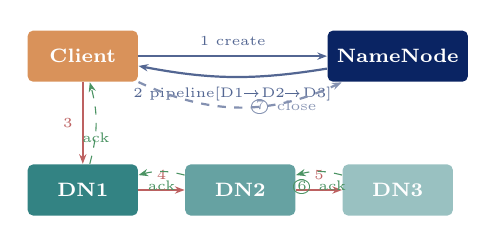
\begin{tikzpicture}[
          actor/.style={rectangle, rounded corners=2pt,
                        minimum width=1.4cm, minimum height=0.65cm,
                        font=\scriptsize\bfseries, align=center},
          arr/.style={-{Stealth[length=3.5pt]}, thick},
          ack/.style={-{Stealth[length=3.5pt]}, dashed, PUGreen!80}
        ]
        \node[actor, fill=PUOrange!70, text=white] (cl) at (0,   4.5) {Client};
        \node[actor, fill=PUNavy,       text=white] (nn) at (4.0, 4.5) {NameNode};
        \node[actor, fill=PUTeal!80,    text=white] (d1) at (0,   2.8) {DN1};
        \node[actor, fill=PUTeal!60,    text=white] (d2) at (2.0, 2.8) {DN2};
        \node[actor, fill=PUTeal!40,    text=white] (d3) at (4.0, 2.8) {DN3};

        % Requests
        \draw[arr, PUNavy!70] (cl) -- node[above, font=\tiny]{1~create} (nn);
        \draw[arr, PUNavy!70] (nn) to[bend left=10]
              node[below, font=\tiny]{2~pipeline[D1→D2→D3]} (cl);

        % Write pipeline
        \draw[arr, PURed!70] (cl) -- node[left, font=\tiny]{3} (d1);
        \draw[arr, PURed!70] (d1) -- node[above, font=\tiny]{4} (d2);
        \draw[arr, PURed!70] (d2) -- node[above, font=\tiny]{5} (d3);

        % Acks back
        \draw[ack] (d3) to[bend right=15]
              node[below, font=\tiny]{\textcircled{6} ack} (d2);
        \draw[ack] (d2) to[bend right=15]
              node[below, font=\tiny]{ack} (d1);
        \draw[ack] (d1) to[bend right=15]
              node[below, font=\tiny]{ack} (cl);

        % Close
        \draw[arr, PUNavy!50, dashed] (cl) to[bend right=25]
              node[right, font=\tiny]{\textcircled{7}~close} (nn);
      \end{tikzpicture}
      \end{center}
  \end{columns}
\end{frame}

%----------------------------------------------------------------
\begin{frame}[fragile]{HDFS in Practice: Key CLI Commands}
  \begin{columns}[T]
    \column{0.52\textwidth}
      \begin{block}{Essential HDFS Shell Commands}
        \vspace{4pt}
        \begin{lstlisting}[language=bash]
# List files in HDFS directory
hdfs dfs -ls /user/data/

# Upload local file to HDFS
hdfs dfs -put sales.csv /user/data/

# Download file from HDFS
hdfs dfs -get /user/data/sales.csv ./

# Read file contents
hdfs dfs -cat /user/data/sales.csv

# Delete file
hdfs dfs -rm /user/data/old.csv

# Create directory
hdfs dfs -mkdir /user/data/2024/

# Check cluster health
hdfs fsck / -files -blocks -locations

# Cluster status report
hdfs dfsadmin -report
        \end{lstlisting}
      \end{block}

    \column{0.45\textwidth}
      \begin{exampleblock}{Useful Admin Commands}
        \vspace{4pt}
        \begin{lstlisting}[language=bash]
# Change replication factor for a file
hdfs dfs -setrep 2 /data/file.csv

# Check NameNode storage info
hdfs dfs -df -h /

# Set quota on a directory
hdfs dfsadmin \
  -setSpaceQuota 500g \
  /user/team_data/

# Safe-mode operations (NN startup)
hdfs dfsadmin -safemode get
hdfs dfsadmin -safemode leave

# Balance data across DataNodes
hdfs balancer -threshold 10
        \end{lstlisting}
      \end{exampleblock}
      \vspace{4pt}
      \begin{alertblock}{HDFS vs POSIX}
        HDFS is \textbf{not} a POSIX filesystem.  No random write support (append-only), no in-place updates, no \texttt{mmap}.  Designed exclusively for \textbf{write-once, read-many} workloads.
      \end{alertblock}
  \end{columns}
\end{frame}

%================================================================
\section{Ivy League Alignment}
%================================================================

\begin{frame}{HDFS in Top University Curricula}
  \begin{columns}[T]
    \column{0.55\textwidth}
      \begin{block}{MIT 6.830 — Database Systems (Madden, Stonebraker)}
        \small MIT uses HDFS/GFS as the canonical case study for \textbf{distributed file system design trade-offs}:
        \begin{itemize}
          \item \textbf{Strong consistency vs.\ availability}: NameNode is a CP system\textemdash consistent but unavailable during NN failure
          \item \textbf{SPOF analysis}: The single NameNode is the main architectural weakness; HA design is a distributed-systems engineering exercise
          \item \textbf{Metadata in RAM}: A deliberate trade-off\textemdash fast access in exchange for memory limits on namespace size ($\approx$1 billion files for 128 GB NameNode RAM)
        \end{itemize}
        \vspace{4pt}
        \textbf{Key exam question at MIT 6.830:}\\
        \textit{``How does HDFS enforce consistency without a distributed lock manager?''} (Answer: \textbf{leases} on open files; NameNode is the sole authority on block locations.)
      \end{block}

    \column{0.42\textwidth}
      \begin{exampleblock}{Harvard CS265 — Big Data Systems (Idreos)}
        \small Harvard's course emphasises the \textbf{storage hierarchy} impact on algorithm design:
        \vspace{4pt}
        \begin{itemize}
          \item HDFS abstracts the disk and network into a \textbf{single storage namespace}
          \item Algorithms must be designed to \textbf{minimise the number of passes} over HDFS data (each full pass = petabytes of I/O)
          \item Harvard uses the concept of \textbf{I/O complexity} as a complexity measure, replacing time complexity for big data algorithms
        \end{itemize}
      \end{exampleblock}
      \vspace{4pt}
      \begin{alertblock}{Stanford CS246 (Leskovec)}
        \textit{``We assume throughout this course that data lives in HDFS and algorithms must process it in a small number of sequential passes.  Random access is forbidden.''}\\[4pt]
        This single assumption drives the entire MapReduce, Spark, and streaming design space.
      \end{alertblock}
  \end{columns}
\end{frame}

%================================================================
\section{Student Assessment Pool}
%================================================================

\begin{frame}{Assessment\textemdash MCQ Set A \hfill\small\textit{CLO1}}
  \begin{exampleblock}{Instructions}
    Select the single best answer.  Correct answers \textbf{bolded} for instructor reference.
  \end{exampleblock}
  \vspace{8pt}
  \begin{enumerate}[\textbf{Q1.}]
    \item What is the \textbf{default block size} in HDFS (Hadoop 2.x and later)?
    \begin{enumerate}[(a)]
      \item 32 MB \quad (b) 64 MB \quad (c) \textbf{128 MB} \quad (d) 256 MB
    \end{enumerate}
  \end{enumerate}
  \vspace{8pt}
  \begin{enumerate}[\textbf{Q2.}]
    \item In HDFS, which component stores the \textbf{metadata} (file-to-block mappings, directory tree, permissions)?
    \begin{enumerate}[(a)]
      \item DataNode \quad (b) \textbf{NameNode} \quad (c) Secondary NameNode \quad (d) ResourceManager
    \end{enumerate}
  \end{enumerate}
  \vspace{8pt}
  \begin{alertblock}{Instructor Notes}
    \textbf{Q1:} Hadoop 1.x default was 64 MB\textemdash students who read older textbooks may choose (b).  The 128 MB default was introduced in Hadoop 2.0.  \textbf{Q2:} Many students incorrectly select ``Secondary NameNode''\textemdash reinforce that it performs checkpointing only, never stores primary metadata.
  \end{alertblock}
\end{frame}

%----------------------------------------------------------------
\begin{frame}{Assessment\textemdash MCQ Set B \hfill\small\textit{CLO1}}
  \vspace{6pt}
  \begin{enumerate}[\textbf{Q3.}]
    \item What is the \textbf{default replication factor} for blocks in HDFS?
    \begin{enumerate}[(a)]
      \item 1 \quad (b) 2 \quad (c) \textbf{3} \quad (d) 5
    \end{enumerate}
  \end{enumerate}
  \vspace{8pt}
  \begin{enumerate}[\textbf{Q4.}]
    \item The \textbf{Secondary NameNode} in HDFS primarily serves as:
    \begin{enumerate}[(a)]
      \item A hot standby that takes over automatically when the primary NameNode fails
      \item \textbf{A checkpoint service that periodically merges the Edit Log with the FsImage}
      \item A dedicated node for storing small file metadata to reduce NameNode load
      \item A load balancer that distributes client read requests across DataNodes
    \end{enumerate}
  \end{enumerate}
  \vspace{8pt}
  \begin{alertblock}{Instructor Notes}
    \textbf{Q3:} Replication factor 3 is the default but students should know it is \emph{configurable} per-file.  \textbf{Q4:} Option (a) is the most common wrong answer and represents the \#1 misconception about HDFS.  Spend class time on this distinction.  Option (b) is the exact correct role.
  \end{alertblock}
\end{frame}

%----------------------------------------------------------------
\begin{frame}{Assessment\textemdash True / False \hfill\small\textit{CLO1}}
  \begin{block}{Instructions}
    State True or False and provide a \textbf{one-sentence justification} for full marks.
  \end{block}
  \vspace{6pt}
  \centering
  \renewcommand{\arraystretch}{1.6}
  \begin{tabular}{p{9.0cm}c}
    \toprule
    \textbf{Statement} & \textbf{Answer} \\
    \midrule
    1.\ HDFS is optimised for low-latency random-access reads of small records. &
    \alert{\textbf{False}} \\
    2.\ The Google File System paper (Ghemawat et al., 2003) directly inspired the design of HDFS. &
    \textbf{True} \\
    3.\ In HDFS, computation (MapReduce tasks) is moved to the nodes that hold the data, rather than moving data to a compute server. &
    \textbf{True} \\
    4.\ If the active NameNode crashes, the Secondary NameNode automatically becomes the new NameNode and the cluster continues without interruption. &
    \alert{\textbf{False}} \\
    \bottomrule
  \end{tabular}
  \vspace{6pt}
  \begin{exampleblock}{Model Justifications}
    \small \textbf{1:} HDFS is optimised for \emph{high-throughput sequential reads} of large files; random access is slow because HDFS blocks are 128 MB and there is no B-tree index.  \textbf{4:} The Secondary NameNode only performs checkpointing; true automatic failover requires the HDFS HA configuration with a Standby NameNode and ZooKeeper.
  \end{exampleblock}
\end{frame}

%----------------------------------------------------------------
\begin{frame}{Assessment\textemdash Descriptive Questions \hfill\small\textit{CLO1}}
  \begin{block}{Instructions}
    Answer each question in \textbf{100--150 words}.  Include a diagram where indicated.
  \end{block}
  \vspace{10pt}
  \begin{enumerate}[\textbf{D1.}]
    \item Explain the \textbf{master/worker architecture} of HDFS.  Identify each component's role and describe what happens to \textbf{under-replicated blocks} when a DataNode fails permanently.
  \end{enumerate}
  \vspace{8pt}
  \begin{enumerate}[\textbf{D2.}]
    \item Why does HDFS use a \textbf{128 MB block size} rather than the 4 KB blocks used by traditional filesystems?  Name one type of workload that \emph{benefits} from large blocks and one that is \emph{harmed} by them (explain why in each case).
  \end{enumerate}
  \vspace{8pt}
  \begin{enumerate}[\textbf{D3.}]
    \item \textbf{Draw and explain} the Hadoop ecosystem stack.  For each of the four layers (HDFS, MapReduce, YARN, Applications), state its role and give one concrete component or tool that belongs to that layer.
  \end{enumerate}
\end{frame}

%----------------------------------------------------------------
\begin{frame}{Assessment\textemdash Analytical Questions \hfill\small\textit{CLO1}}
  \begin{block}{Instructions}
    Answer in \textbf{200--300 words} with step-by-step reasoning.  Marks awarded for correct process, not just conclusion.
  \end{block}
  \vspace{6pt}
  \begin{enumerate}[\textbf{A1.}]
    \item \textbf{Replication Recovery Trace:}\\
    A DataNode (DN4) that stores the \textbf{only} copies of blocks B7, B8, and B9 crashes permanently (it was hosting the 2nd replica of B7 and 3rd replica of B8, but the \emph{only} replica of B9\textemdash the other DataNodes holding B9 also failed earlier).
    \begin{itemize}
      \small
      \item What does the NameNode do for B7 and B8 (under-replicated)?
      \item What is the situation for B9, and what does this mean for data that relied on it?
      \item How does the rack-aware replication policy determine \emph{which} DataNodes receive the new replicas of B7 and B8?
    \end{itemize}
  \end{enumerate}
  \vspace{6pt}
  \begin{enumerate}[\textbf{A2.}]
    \item \textbf{HDFS vs.\ NFS:}\\
    A university wants to store 50 TB of genomics research data that will be analysed by Spark jobs (sequential scans) but also queried interactively by individual researchers (random access to specific gene records).  Compare HDFS and NFS on four dimensions (scale, fault tolerance, access pattern, cost) and recommend the appropriate system.  Could a hybrid approach work?  Justify.
  \end{enumerate}
\end{frame}

%================================================================
\section*{Textbook References}
%================================================================

\begin{frame}{Textbook \& Reading References}
  \begin{block}{Primary Textbooks for Week 3}
    \begin{itemize}
      \item \textbf{[TW]}\ Tom White. \textit{Hadoop: The Definitive Guide}, O'Reilly, 4th ed., 2015.
            \hfill \textbf{Chapters 1, 3}
            \begin{itemize}
              \small\item Ch.\,1: Meet Hadoop (motivation, history) $\cdot$ Ch.\,3: HDFS (architecture, read/write, HA)
            \end{itemize}
      \item \textbf{[SA]}\ Acharya \& Chellappan. \textit{Big Data and Analytics}, Wiley, 2015.
            \hfill \textbf{Chapter 3}
      \item \textbf{[TE]}\ Erl, Khattak \& Buhler. \textit{Big Data Fundamentals}, Prentice Hall, 2016.
            \hfill \textbf{Chapter 8}
    \end{itemize}
  \end{block}
  \vspace{6pt}
  \begin{exampleblock}{Supplementary (Covered in Week 3, Part 2 — Seminal Paper)}
    \begin{itemize}
      \small
      \item Ghemawat, S., Gobioff, H., \& Leung, S.-T. (2003). \textbf{The Google File System.}
            \textit{ACM SOSP}, pp.\ 29--43. \textbf{[PRIMARY SEMINAL PAPER]}
      \item Shvachko, K., Kuang, H., Radia, S., \& Chansler, R. (2010). \textbf{The Hadoop Distributed File System.}
            \textit{IEEE MSST}. \textit{[How the GFS design was adapted for open-source Hadoop]}
    \end{itemize}
  \end{exampleblock}
  \vspace{4pt}
  \begin{alertblock}{Strongly Recommended Online Resource}
    \small HDFS Architecture Guide (Apache official documentation):\\
    \texttt{https://hadoop.apache.org/docs/stable/hadoop-project-dist/hadoop-hdfs/HdfsDesign.html}
  \end{alertblock}
\end{frame}

%----------------------------------------------------------------
\begin{frame}[c]
  \begin{center}
    {\Large\bfseries Questions \& Discussion}\\[10pt]
    {\large Week 3, Part 1 $\;\mid\;$ CSE 4345 Big Data Analytics}\\[8pt]
    \textcolor{PUGray}{\rule{7cm}{0.5pt}}\\[10pt]
    \begin{quote}
      \itshape ``We have found that at our scale, the most effective approach to fault tolerance
                 is the ruthless elimination of single points of failure, not heroic individual components.''}
    \end{quote}
    \hfill\textemdash\,Sanjay Ghemawat, Google File System (2003)
    \vspace{14pt}
    \begin{block}{\centering Next Lecture: Week 3, Part 2}
      \centering
      Seminal Paper: Ghemawat, Gobioff \& Leung (2003) — \textit{``The Google File System''}\\[4pt]
      \small Design principles $\cdot$ Chunk management $\cdot$ Consistency model $\cdot$ Master recovery\\
      Case Study: Yahoo!'s 10{,}000-node Hadoop deployment (2008)
    \end{block}
    \vspace{6pt}
    \textbf{Reading before Part 2:}\ \textbf{[TW]} Ch.\,1 \& 3 $\cdot$ GFS paper (see reference slide)
  \end{center}
\end{frame}

%=================================================================
\end{document}
%=================================================================
